\documentclass{article}%
\usepackage[T1]{fontenc}%
\usepackage[utf8]{inputenc}%
\usepackage{lmodern}%
\usepackage{textcomp}%
\usepackage{lastpage}%
\usepackage{geometry}%
\usepackage{float}%
\usepackage{biblatex}%
\usepackage{hyperref}%

\addbibresource{citations.bib}
\geometry{tmargin=1cm,lmargin=0.75cm,rmargin=0.75cm}%
\usepackage{graphicx}%
\setlength{\parskip}{0.2em}%
%
\title{The Stern Gerlach experiment and estimating the magnitude of the Bohr magneton, $\mu_\beta$.}%
\date{}%
%
\begin{document}%
\maketitle
\section*{Abstract}
In this report I aim to replicate the findings of the Stern Gerlach experiment. Further, using 
measurements from a separate lab group as we could not get usable data from our apparatus,
I estimate the $\mu_{\beta} = (4.79 \pm 1.03) \times 10^{-24} JT^{-1}$. I offer some explainations for the differences
between the result and the accepted value in the literature and how these may be tested and rectified.
\section{Introduction}
\subsection{Historical background}
The Stern Gerlach experiment \cite{SG} was performed in an attempt to corroborate the Bohr-Sommerfeld model's prediction that the direction of the angular momentum in a silver atom is quantized.
It was successful in this attempt in what was said to be the 'last hurrah of the old quantum theory' \cite{Baggot}. 
\paragraph{}
The classical expectation was to find one peak on the detector. In fact, two peaks were found for the silver atom providing what was deemed experimental evidence for angular momentum quantization in all atomic systems.
Despite the decline of the Bohr theory, the Stern Gerlach has been shown to agree with further developments in quantum theory. 
The orbital angular momentum of a the silver atom is actually zero, wrongly presumed to be $\frac{h}{2\pi}$ in the Bohr model. The magnetic moment is due solely to a half unit of spin angular momentum accounting for the twofold splitting.
However at the time of the experiment, Stern and Gerlach "had no idea it was spin that they had discovered" \cite{PT}. The earliest attribution of the splitting effect to spin came in 1927 by Ronald Fraser \cite{Fraser}. 
\paragraph{}
Otto Stern subsequently won the Nobel prize in 1943 "for his contribution to the development of the molecular ray method and his discovery of the magnetic moment of the proton." \cite{Nobel}
\subsection{Theoretical background}
A simplified sketch of the Stern Gerlach apparatus is shown in figure 1 below.
\begin{figure}[H]%
    \centering%
    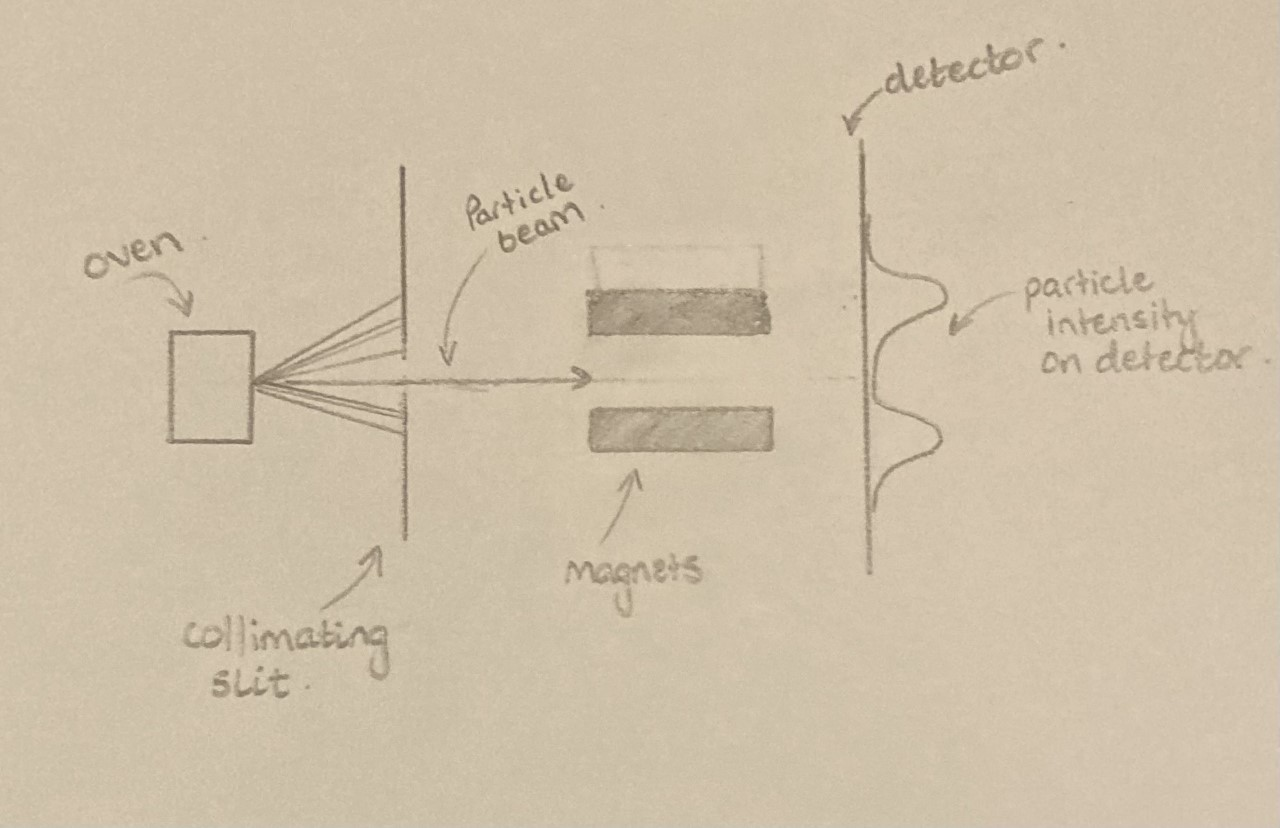
\includegraphics[width=300px]{simply_sg.png}%
    \caption{Simplified diagram of the Stern Gerlach experiment.}%
\end{figure}

An oven containing a potassium is heated. By collision in the oven particles are projected outwards and some pass through the collimated slits producing a beam of potassium atoms.
As the particles move down the vacuum containing the apparatus, they experience a force due to the magnetic field created by the electromagnet. 
This force acts because the potassium atom has one unpaired valence shell electron and therefore has a net magnetic dipole moment or "spin". 

The force acting on the particle due to the magnetic field, B can be given as


\begin{equation}
    \vec{F} = \nabla(\vec{\mu} \cdot \vec{B} )
\end{equation}

However, as we are only considering the z-component of the potassium atoms motion i.e. the line in which the detector sits, we can consider only the force acting in the z direction,

\begin{equation}
    F_z = \mu_z \frac{dB}{dz}
\end{equation}

The direction of the force experienced by the particle can be either positive or negative depending on the direction of $\mu_z$ 
This means the force can act both upwards and downwards in the particle depending on the direction of it's spin.
This is represented by the two peaks on figure one. Potassium atoms of different spin states are deflected forming the distrubution with two peaks on the screen.
Identical particles would be deflected by the same amount meeting at a two points on the detector given that the magnetic dipole moment is quantized and can only take on discrete values.
However, as the atoms have a range of velocities after being ejected from the oven they will experience different impulses due to the field i.e. the time under the action of the force and so deflect by different amounts.
We will then estimate the peaks of the distrubution to be these points.

If we assume that N particles from the furnance have velocities that follow a Maxwell-Boltzman distribution 


\[ \scalebox{1.5}{$N(\Delta) \propto (\Delta Z)^{-3} e^{\frac{-F_z \cdot L(l- \frac{L}{2})}{2 \Delta z kT}}$} \]
Where l is the distance between the start of the magnets and the detector, L is the distance over which the potassium atom experiences the magnetic force, k is the Boltzman constant and T is the temperature of the oven.
To find the maxima of this function and hence the most probable place to detect a potassium atom we can differentiate the expression


\[ \scalebox{1.5}{$\frac{dN}{dz} =  e^{\frac{-F_z \cdot L(l- \frac{L}{2})}{2 \Delta z kT}} \cdot (-\frac{3}{(\Delta Z)^4} - \frac{1}{(\Delta Z)^5}) = 0 $} \]

$\Delta Z = -3$ and so  

$$
\frac{-F_z \cdot L(l- \frac{L}{2})}{-6 \cdot \Delta z_p kT} = 1 
$$

Therefore 
\begin{equation}
    \Delta Z_p = \frac{\partial B}{\partial z} \cdot \frac{\mu_z \cdot  L(l - \frac{L}{2})}{6kT}
\end{equation}

We can proceed with the experiment and measure $\mu_z$, the component of the magnetic dipole in the z axis.

\section{Methods}
Figure 2 shows the experimental setup. 
\begin{figure}[H]%
    \centering%
    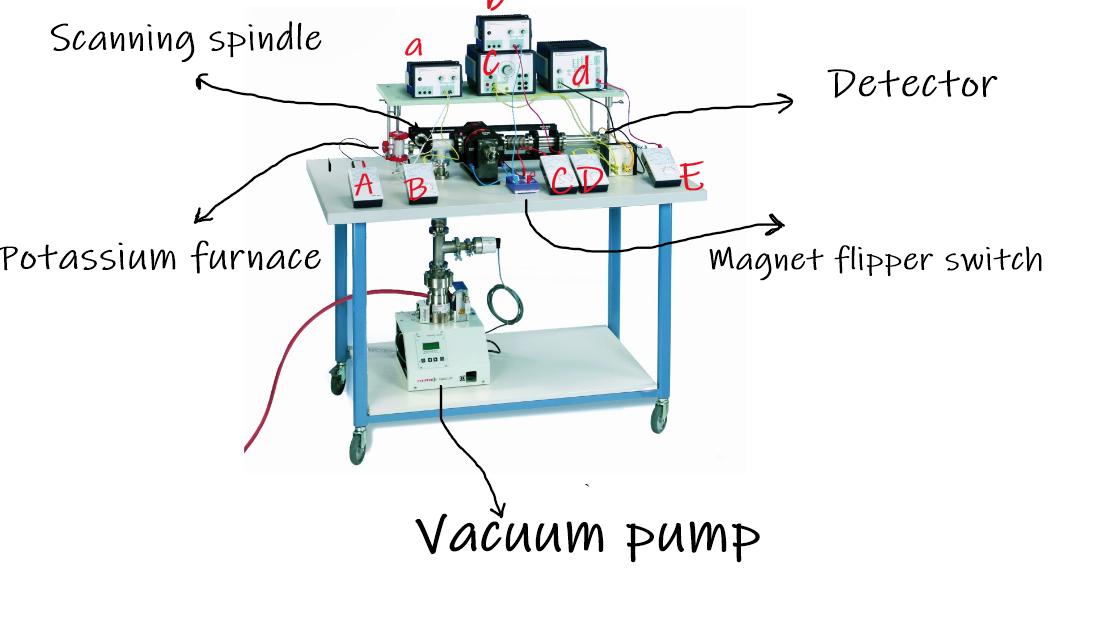
\includegraphics[width=400px]{experimental_setup_labeled.png}%
    \caption{Experimental setup used to replicate the Stern Gerlach experiment. Image [\url{https://www.phywe.com/experimants-sets/nobel-prize-trials/stern-gerlach-experiment_9233_10164/}]}%
\end{figure}
The potassium furnance on the left is heated using the 'a' power supply and measured from the meter 'A'. A fraction of the evaporated potassium atoms are sent down towards the detector and are collimated into a beam.
An electromagnet sits in between the potassium furnance and the detector. By changing the input current on 'c' we can change the strength of the magnetic field generated by the electromagnet. The potassium atoms can then be detected using readings from ammeter 'E'.
This detector makes use of power supply 'd' to amplify the current in the dector for possible observation.
By varying the scanning spindle and recording the distribution of currents in the detector we can get a graph as follows:

\begin{figure}[H]%
    \centering%
    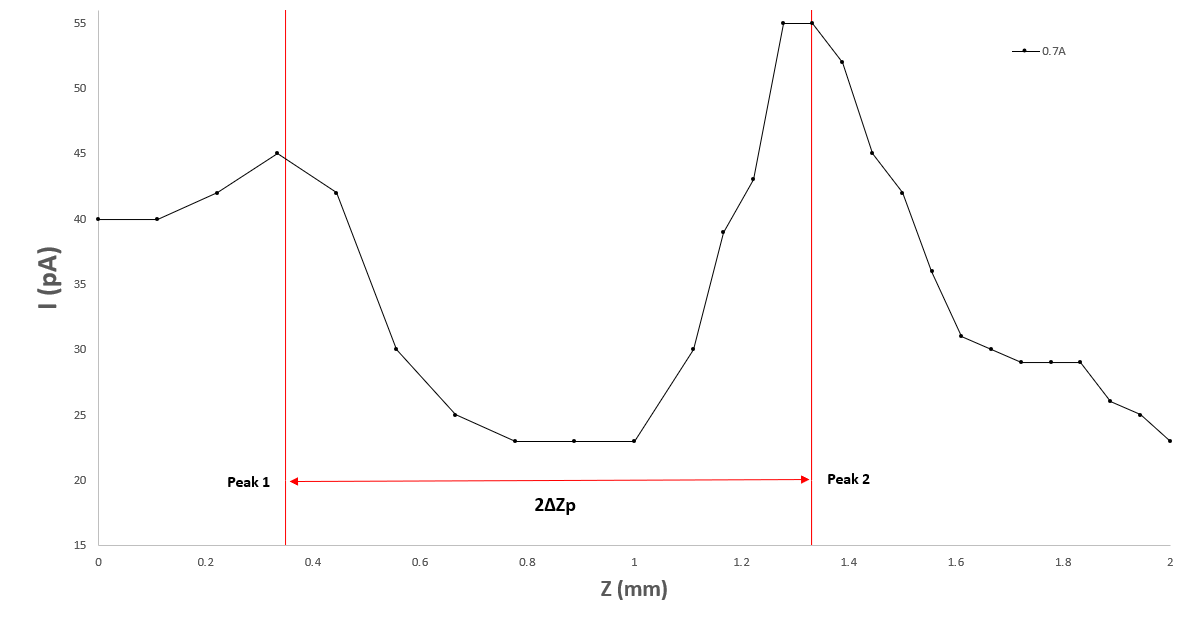
\includegraphics[width=300px]{graph_3.png}%
    \caption{Distribution of values for a current in the electromagnet of 0.7A.}%
\end{figure}
The red lines show the width between the peaks which we can estimate to be $2\Delta Z_p$.
\paragraph{}
The accompanying experimental manual provided by the manufacturer provides specific data for the field inhomogeneities at different excitation currents according to the calibration curves of the magent \cite{PHYWE}. 
In order to extract the necessary values for this experiment, I plotted these values in figure 4. Using linear regression I was able to develop an equation for the relationship between the current and the field inhomogeneity.
\begin{equation}
    \frac{\partial B}{\partial z} = 308.69 I + 2.21 
\end{equation}

It was then possible to find the error in this gradient
\begin{equation}
    \sigma_m = \sigma_{CU} \sqrt{\frac{N}{\Delta}}    
\end{equation}
Here, $\sigma_{CU}$ is the common uncertainty, N is the number of data points and $\Delta$ is 

$$
\Delta = N \sum_{i=1}x_i^2 - (\sum_{i=1}x_i)^2
$$
I could then estimate $\sigma_m = \pm 1.48 kgs^{-2}A^{-2}$
\begin{figure}[H]%
    \centering%
    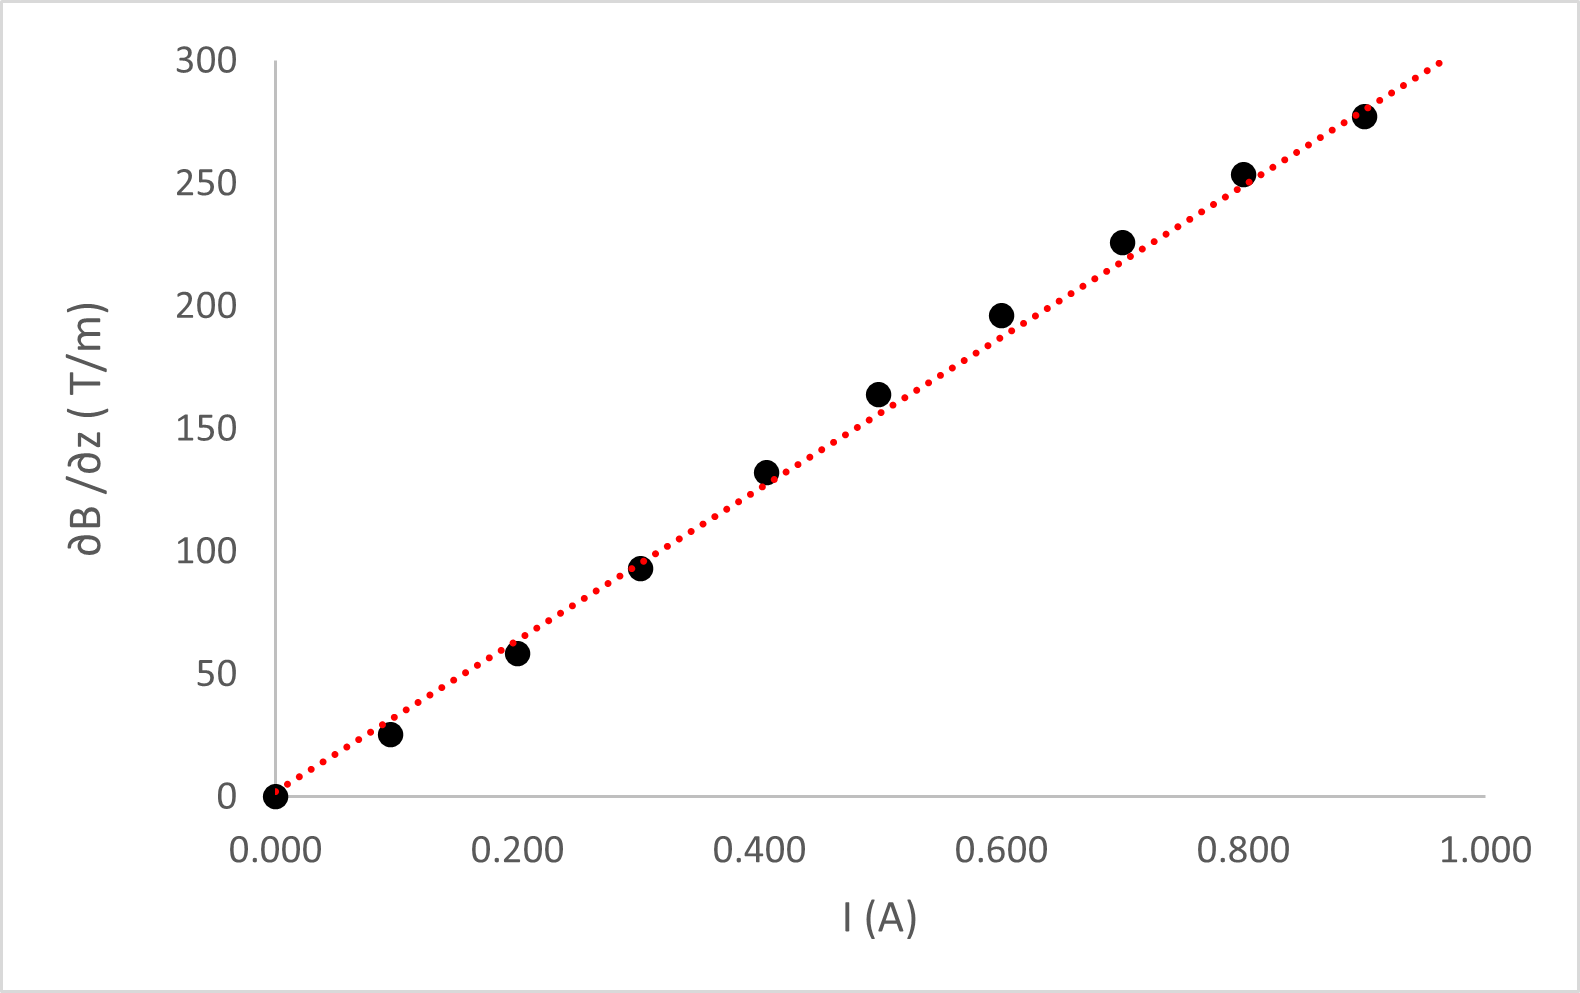
\includegraphics[width=400px]{graph_2.png}%
    \caption{Plot of the configuration data provided by PHYWE.}%
\end{figure}
\section{Results}
\begin{table}[H]
    \begin{centering}
    \begin{tabular}{|p{3cm}||p{3cm}|p{3cm}|p{3cm}|} 
        \hline
        Current / A & $\Delta Z_{p}$ / mm & $\overline{\sigma}_{\Delta Z_{p}}$ / mm & $\frac{\partial B}{\partial z}$ / $Tm^{-1}$ \\ [0.75ex] 
        \hline\hline
        0.50 & 0.445 & 0.134 & 156.37 \\ 
        \hline
        0.75 & 0.468 & 0.076 & 233.54 \\
        \hline
        0.90 & 0.784 & 0.136 &  279.84 \\
        \hline
    \end{tabular}
    \caption{Results from the measured peaks. Current as measured as input into the electromagnet, $\Delta Z_{p}$ and the average uncertainty is measured from the subsequent plots of current on spindle position, asymmetrical uncertainties are preserved for the plots. $\frac{\partial B}{\partial z}$ is iterpolated from the calibration curve provided. }
\end{centering}
\end{table}

\begin{figure}[H]%
    \centering%
    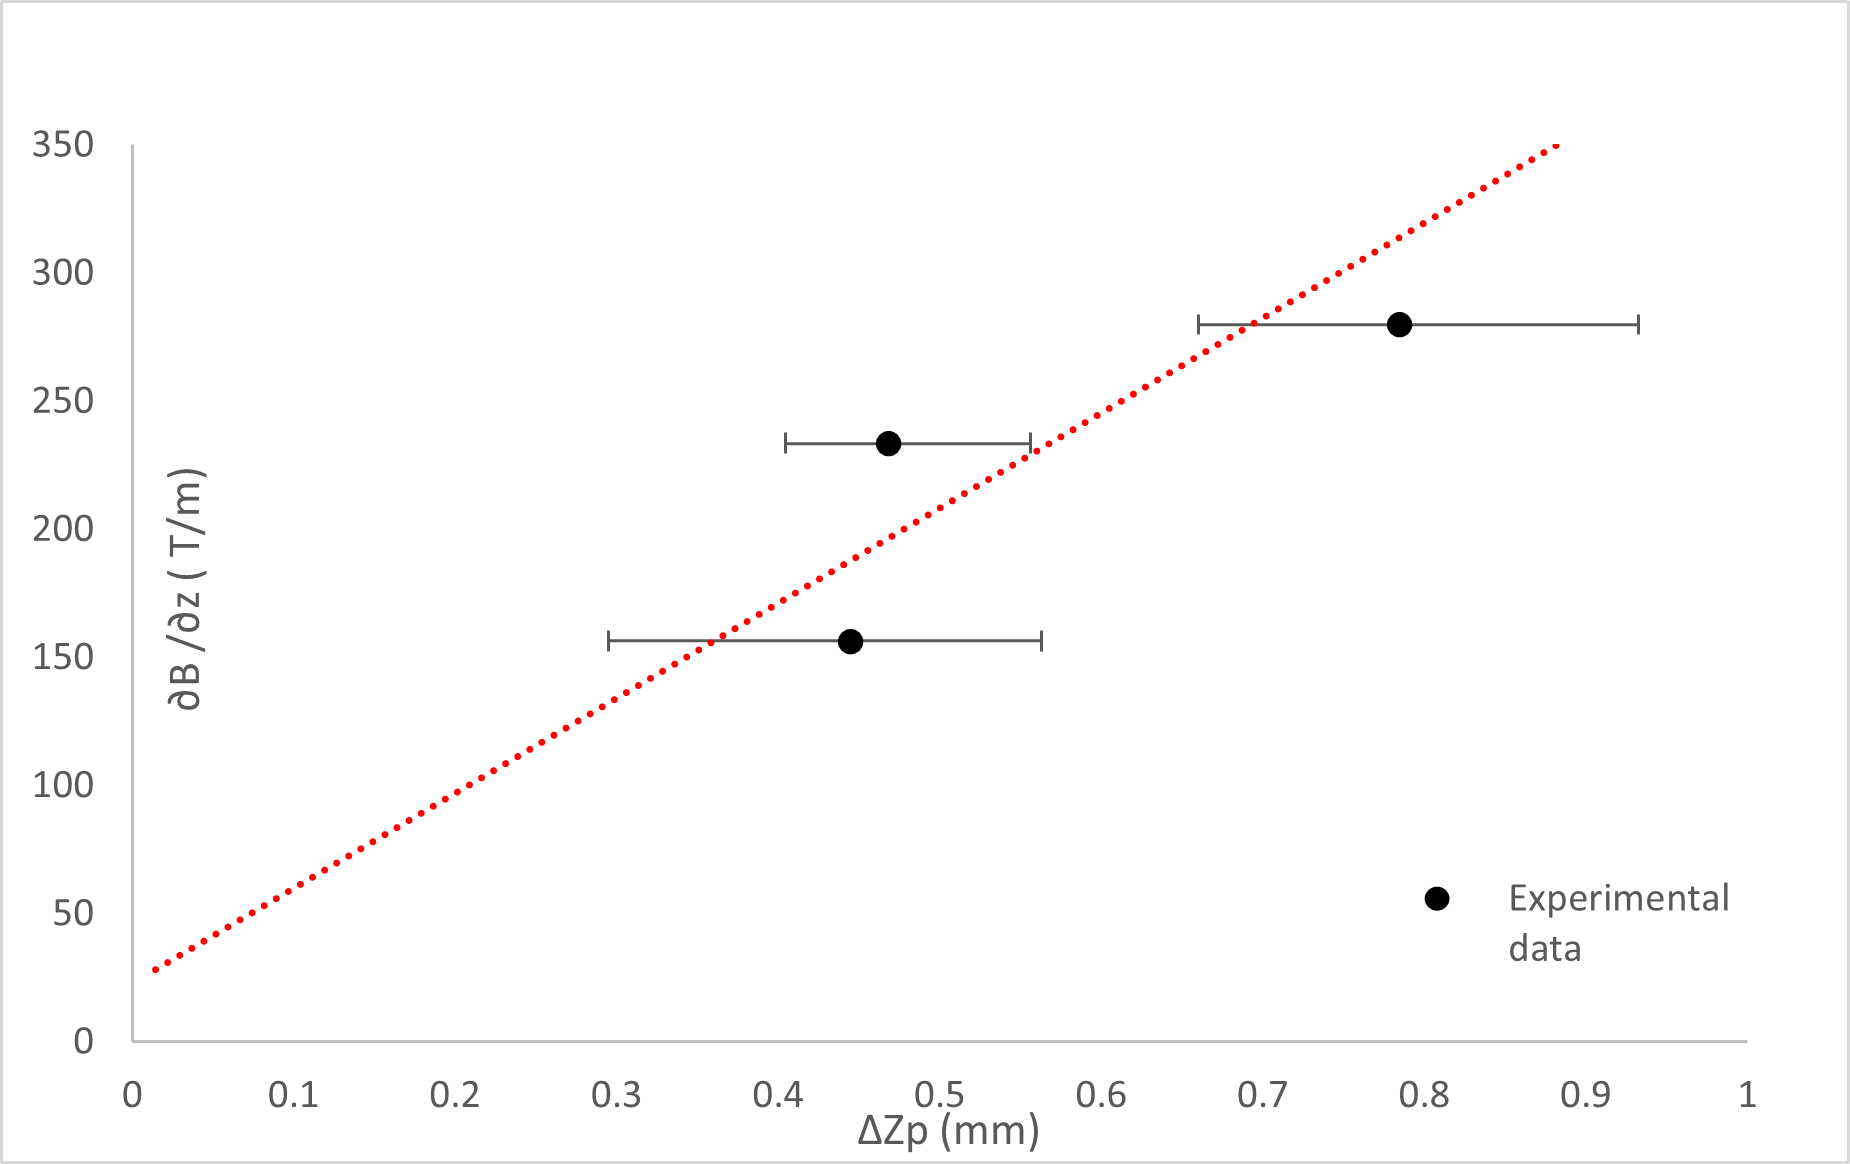
\includegraphics[width=400px]{graph_1.png}
    \caption{Plot of $\frac{\partial B}{\partial z}$ on $\Delta Z_{p}$.}%
\end{figure}

\section{Analysis}
\subsection{Calculation of $\mu_{\beta}$}
From the rearrangment of equation (1) we can calculate the gradient of figure 5, m as 
$$
    m = \frac{6kT}{\mu_z \cdot L(l - \frac{L}{2})}
$$
This will allow a measurement of $\mu_z$.

The Bohr magneton is given by 
\begin{equation}
    \mu_{\beta} = \frac{\pm 2 \mu_{z}}{g_s}
\end{equation}


This allows us to state  $\mu_\beta$ in terms of our gradient and the provided constants.

\begin{equation}
    \mu_{\beta} = \frac{12kT}{m \cdot L(l - \frac{L}{2})}
\end{equation}

\subsection{Calculation of the uncertainty in $\mu_{\beta}$}
Firstly, it is important to calculate the uncertainty in the gradient of figure 5, which combines the uncertainties in the field inhomogeneity and the distance between peaks. It is evident by inspection of the graph that the uncertainty in $\Delta Z_p$ is dominant. We can again use equation (5) to find the uncertainty in this gradient.

In order to determine the uncertainty in the value of $\mu_{\beta}$, $\sigma_{\mu_{\beta}}$ we can use the calculus based method combine the uncertainties to get

$$
\sigma_{\mu_{\beta}}^2 = ( \frac{\partial \mu_{\beta} }{\partial m}  \cdot \sigma_{m})^2 + ( \frac{\partial \mu_{\beta} }{\partial L}  \cdot \sigma_{L})^2 + ( \frac{\partial \mu_{\beta} }{\partial l}  \cdot \sigma_{l})^2
$$

From the above we can determine $\mu_{\beta} = (4.79 \pm 1.03) \times 10^{-24} JT^{-1}$.

\subsection{Discussion of the result for $\mu_\beta$} 
The accepted value in the literature is $\mu_\beta$ = 9.27 $\times 10^{-24} JT^{-1}$. \cite{NIST}
 As our result is more than three standard errors from the accepted value then we must conclude that our result is in disagreement with the literature.
One major factor is the lack of data points. With a small sample size our result will be vulnerable to large random errors, so it is important to increase the number of measurements to rule out this possibility for error. 
\paragraph{}
Another factor is human error in the readings of the data. What is notable on figure two is the closeness of data points for I = 0.50A, 0.75 A on the x axis. This suggestes a reading error from the scales. To rule out this possibilty, we should repeat these readings to determine if such an error was made.
From an analytical point this makes sense as $\mu_\beta \propto \frac{1}{m}$, if the second data point was erroneous to the upside this would increase the gradient and decrease the measured value of $\mu_\beta$ explaining why our value is lower than expected. 
Again, these types of errors will be compounded using a small dataset.

\section{Conclusion}
In this experiment, I was able to repeat the Stern Gerlach experiment and observe the evidence for the quantized magnetic moment of the potassium atom from the peaks evidenced in figure 3.
I was also able to derive the relationship between this peak distance and the Bohr Magneton and estimate it to be $\mu_\beta = (4.79 \pm 1.03) \times 10^{-24} JT^{-1}$. I have also discussed the limitations in our experimental method. I have suggested methods for testing these limitations in order to explore further the discrepancy between the result and the accepted value.
\printbibliography
\end{document}